% 2013 年安徽卷文科第 18 题：四棱锥 P-ABCD，底面 ABCD 是菱形，E 为 PA 中点。
% 来源 PDF：普通高考/2013/2013安徽文.pdf，第 2 页（印面 786）左栏。
% 底面菱形按斜二测投影画出：A 左、B 前、C 右、D 后；D 与 PD 被遮挡。
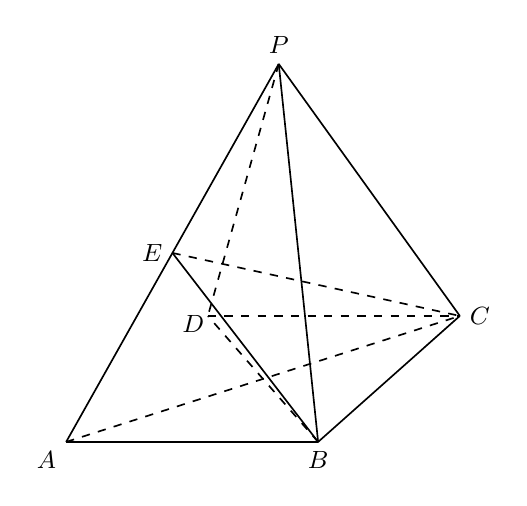
\begin{tikzpicture}[semithick, font=\small]
  \coordinate (A) at (0,0);
  \coordinate (B) at (3.2,0);
  \coordinate (C) at (5.0,1.6);
  \coordinate (D) at (1.8,1.6);
  \coordinate (P) at (2.7,4.8);
  \coordinate (E) at (1.35,2.4);
  % 可见棱
  \draw (P) -- (A);
  \draw (P) -- (B);
  \draw (P) -- (C);
  \draw (A) -- (B) -- (C);
  \draw (E) -- (B);
  % 被遮挡的棱与辅助线
  \draw[dashed] (P) -- (D);
  \draw[dashed] (D) -- (C);
  \draw[dashed] (A) -- (C);
  \draw[dashed] (B) -- (D);
  \draw[dashed] (E) -- (C);
  % 标注
  \node[above] at (P) {$P$};
  \node[below left] at (A) {$A$};
  \node[below] at (B) {$B$};
  \node[right] at (C) {$C$};
  \node[left, yshift=-3pt, fill=white, inner sep=1pt] at (D) {$D$};
  \node[left] at (E) {$E$};
\end{tikzpicture}
